\section{\tool}
\label{sec:badusb}
\subsection{Threat Model}

We build our threat model on the basic assumptions that common users without
technical background would not treat normal-looking USB device as highly
dangerous and be cautious about them. These assumptions are approved in a
relevant work about charging attack~\cite{JFCImpact}. Moreover, we neglect the
effect of notification about common USB device, as normal users usually are not
equipped with the necessary knowledge to fully understand such notices. In
fact, during our experiment, no device had security notifications raised about
suspicious USB devices and only mobile devices had raised charging notification
about our \tool, which may not be a sufficient warning towards users.

We also assume the victim's device is equipped with fully functional USB 3.x
protocol and USB Type C connector. As the USB 3.x standard is more and more
common nowadays, this assumption can be easily fulfilled especially in recent
devices.

%\subsection{Motivation}
%\noindent\outline{Limitation of Rubber Ducky}\\
%\outline{Our functionality different mode listing?}\\
%\hongyi{The following mode is to be further decided}
%\outline{Automatic Scripting Mode}\\
%\outline{Remote Control Mode}\\
%\outline{OCR/QR Recognition Mode}\\

\subsection{Implementation}
%\noindent\hongyi{The following mode is to be further decided}\\
%\outline{DETAIL of each mode}\\ \outline{Automatic Scripting Mode}\\
%\outline{Remote Control Mode}\\ \outline{OCR/QR Recognition Mode}\\
As we introduced in Section~\ref{sec:related_work}, there are plenty of
existing work~\cite{rubber,badusb,
rubberducky2020,usbbypassing,iseeyou,usbdriver} focusing on BadUSB attack.
Many of these take advantage of the \textit{trust-by-default} policy of PC,
pretend to be normal HID devices and utilize USB protocol to perform attacks.
However, these attacks suffer from various drawbacks: \ding{182} attackers can
only simulate limited types of devices such as HIDs (like keyboards and mice)
and disks, which makes the attacks less effective; \ding{183} accurate attacks
could not be performed due to lack of user interface (UI).  Whatever HID the
attackers simulate their USB devices to be, they could not obtain the UI to
check the current situation, which makes it nearly impossible to carry out
their attacks precisely or confirm the effects after attacks.

In this work, we utilized the new features of USB 3.x~\cite{usb31,usb32} to
address the problems above.  Benefiting from latest protocol, we simulated
external display and thus obtained the video stream to perform accurate
attacks.

%Though BadUSB devices\cite{badusb} like Rubber Ducky\cite{rubber,
%rubberducky2020} emulates as a HID device enabling various arbitrary execution
%attacks, fetching feedback from the victim is much more limited.
Based on the drawbacks introduced above, several defense mechanisms were
proposed, like GoodUSB~\cite{tian2015defending}. These defense mechanism
implemented a CAPTCHA-like~\cite{captcha} procedure, which requires user to
complete certain challenges when an unknown HID device is plugged in. As the
BadUSB is only able to emulate a limited kind of devices like HID or disks, by
no means the BadUSB can bypass it. Our \tool, on the other hand, is capable of
bypassing this type of defense. Taking advantage of USB 3.x~\cite{usb31,usb32},
\tool can fetch the video stream of the victim and complete the challenge
manually by the attacker. Moreover, with video capability combined with
traditional BadUSB, our \tool achieved multiple new attack paradigms and are
tested under various real-world scenarios.

As there were various BadUSB implementations available, we only focus on its
core functionality and our extension. In this section, we first introduce the
components we used in \tool, then we focus on the three different attack modes
we implement for various scenarios.

\subsubsection{Attack Model}

The components in our attack model are as follows, and the relation between
them is illustrated at Figure~\ref{fig:attack_model}. \fengwei{We need to
explain the figure. What are the boxes? Where is victim? Where is the attacker?
The list below only shows the internal components in the malicious USB device.
We might also consider to explain this in the Figure caption.}

\begin{itemize}
	\item\textit{USB 3.x Hub} exports the USB 3.x connector into various ports, like DisplayPort, USB 2.0 port etc.
	\item\textit{Video Capture Card} convert DisplayPort signal into UVC-compatible\hongyi{citation needed} data, which is later processed by embedded computer.
	\item\textit{Single Board Computer} processes video stream from the victim where private data is extracted and transmitted via GSM/WiFi to the attacker.
	\item\textit{HID Emulator} emulates HID device which can be controlled from the attacker.
\end{itemize}


\begin{figure}[t]
	\centering
	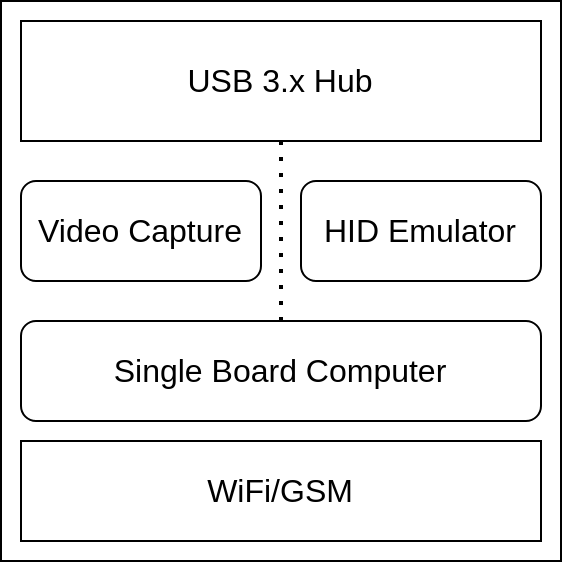
\includegraphics[width=\linewidth]{./Figs/attack_model.png}

	\begin{tabular}{ll}
	\mycircled{1}Victim's Device    &\mycircled{2}\tool\\
	\mycircled{3}Attacker's Device
	\end{tabular}

	\caption{Attack Model}%\shuqing{Need to be more compact.}
	\label{fig:attack_model}
\end{figure}

\textbf{Scripting Mode.} This mode majorly relies on the ``HID Emulator'' to
send constructed HID packet to the victim. These constructed HID packets are
interpreted by the victim as valid keystrokes and mouse moves. Thus, the
attacker can executes arbitrary scripts on the victim's device. This is the
function of the original BadUSB. Based on this, we made the following
improvement.

First, \tool supports defense-bypassing. As the original BadUSB cannot get
feedback from the victim, defense mechanisms like GoodUSB
\cite{tian2015defending} are sufficient to prevent these BadUSB attacks.
However, these defense mechanisms leverage visual notification to block access
for unknown USB devices. This means that when the defense request authorization
from the user, our \tool is able to capture the content of authorization
challenge and bypass it. After the defense is bypassed, \tool continues the
emulation and script execution, resulting in a successful attack.

Moreover, as the mouse relies on the visual feedback to work properly, its
emulation and automation were not supported by the original version of BadUSB.
Yet with the video output support from USB 3.x, our \tool implements
full-functional mouse emulation. This function enables attacks toward pure GUI
programs and shows great potential in the mobile attack scenario. Details can
be obtained in Section~\ref{sec:experiment}.

The advantage of this mode is that it archives defense bypass and attack
feedback with video streaming.  \fengwei{I don't understand the sentence below.}\hongyi{Fixed, I think it's redundant and less important}
%As mentioned above, we only require video stream at the beginning (defense
%bypass) and the end (result feedback) of the attack.
Moreover, with mouse
supported, \tool extends the original BadUSB attack surface and perform well in
mobile device.

\textbf{Privacy Extraction Mode.} \tool under this mode does not emulate other
USB device and solely relies on the video stream function of USB 3.x; it uses
``Video Capture'' component to transmit the stream to embedded ``Single Board Computer''\fengwei{What is embedded computer? Do we define this in the previous\hongyi{Fixed by using the term mentioned in Figure}
text?}. The victim's device would mistakenly treat \tool as an external monitor
and output its video stream. This stream is latter processed by the embedded
computer to extract private data.

When running in this mode, \tool passively processes the victim's video stream
and detect for ``valuable'' private data.  The data is considered as
``valuable'' or not is decided by a customized detector, we implement a simple
payment code detector for the demonstration purpose. Though this detector is
simple to implement, we successfully transfer money from the victim to the
attacker. More detail can be obtained in Section~\ref{sec:experiment}.

It is worth mentioning that \tool under this mode is completely passive, making
it hard to be detected and defended. With different detector implemented, \tool
under this mode is capable of serving more purposes.

\textbf{Remote Control Mode.} In \tool, we have implemented all components
required to control a computer/mobile device remotely, including a video stream
and a keyboard/mouse emulation. Thus with all components enabled, not only will
the victim's device treat \tool as an external display, but also a valid HID
input source. Hence we can archive complete hijack of victim's device.

\tool under this mode follows a simple logic. \tool will receive video stream
from the victim's device and redirect it to the attacker via GSM/WiFi. In the
meanwhile, \tool also receives keystrokes and mouse movement from the attacker
through GSM/WiFi and replay them to the victim by the USB emulation.

This mode enable attacker to perform delicate operation that is beyond
automation. Moreover, this mode provides a backdoor that does not require host
network and thus is undetectable by the firewall running on the host machine.
%\hongyi{I think this is a quite good selling point?}\shuqing{Agree with
%Hongyi.}

The advantage of this mode is that it can completely hijack the victim device
and provide a backdoor beyond detection of firewalls. But this complete control
also comes with the price of high power consumption and risk of being detected
by the user.

